
\section{Introduction} \label{intro}

Hardware HEVC encoders have recently appeared on consumer-grade GPUs, opening the door to mass live $360\,^{\circ}$ video streaming. Traditional methods of adaptive bitrate (ABR) streaming, however, do not work on these ultra-high resolution videos because the bitstream will either be too large for continuous playback or of too low a quality to be enjoyable. A body of work on tile-based ABR streaming for UHD video has recently appeared in which the quality requested for each section of a video corresponds to the current or predicted viewport, allowing end-users to view the most important parts of a video in high-quality without stalling \cite{lefeuvre2016,corbillon2016,PetrangeliSHT17}. This is straightforward for pre-rendered videos, but is more complicated in live streaming because each quality requires a different encode, introducing some delay in the availability of each new segment. Furthermore, tiling is not supported by existing hardware encoders. One may feed each tile to the encoder as a separate video and stitch them together afterwards, but the cropping required on each frame introduces considerable overhead.

To combat these challenges, we introduce RATS, a GPU-based HEVC encoding platform to tile, encode, and stitch 360 video at multiple qualities in real-time. The source video stream is divided into columns which are stacked on top of one another. The rearranged video image is then fed to the hardware encoder with slice boundaries set at the edges of the source video. This process occurs twice for each frame, once with a low average bitrate and once with a high one. When the video is reconstructed during playback, each tile is an independent region, allowing us to pick where every tile (belonging to either bitstream) should appear in the final video.

The rest of this paper is organized as follows. In Section \ref{hevc}, we provide background on HEVC and the NVENC hardware encoder. In Section \ref{rats}, we describe the proposed system in detail. In Section \ref{infra}, we sketch out a full web-based video streaming platform centered around RATS. In Section \ref{eval}, we provide an evaluation of the system. Finally, Section \ref{concl} concludes the work.

\renewcommand{\figurename}{Fig.}
\begin{figure*}[t]
	\centering
	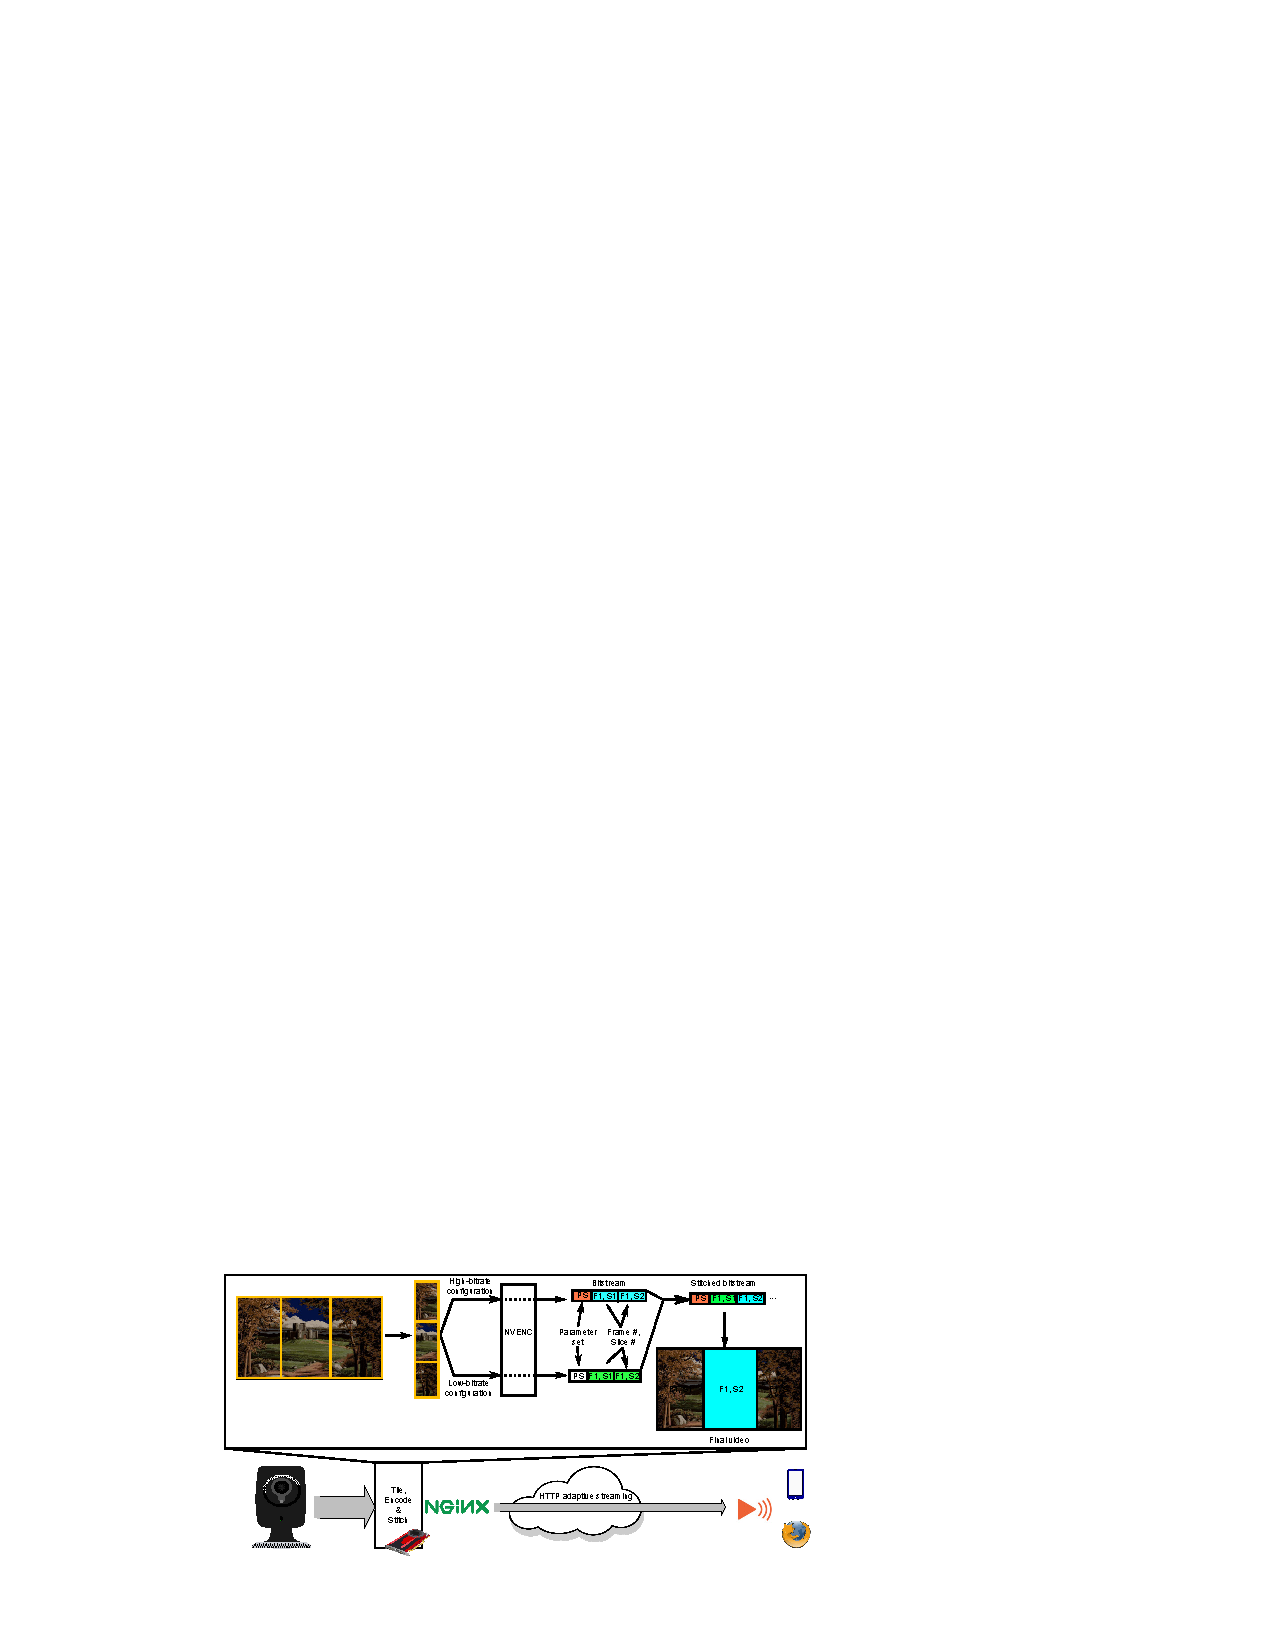
\includegraphics[width=0.8\textwidth]{figures/Streaming_scenario_v3.pdf}
	\caption{Adaptive $360\,^{\circ}$ Live Streaming. In this demo we show hardware encoding that allows us to stitch single tiles of the $360\,^{\circ}$ video in different quality levels (see expanded pipeline). The lower part of the figure shows the demo setup in a streaming infrastructure that makes use of HTTP adaptive streaming.}
	\label{fig:pipeline}
\end{figure*}

\section{HEVC and NVENC} \label{hevc}

HEVC, also known as H.265, is a modern video compression standard capable of dramatically shrinking video file size without sacrificing quality. Encoding an HEVC video is a computationally expensive process which is not easily parallelized. Instead, encoders divide each frame of the video into independent regions and encode them separately, joining their edges to form the full image during playback. Two functionally identical versions of this concept, slices and tiles, exist within the HEVC standard, but slices are limited to chunking the video into wide strips while tiles can divide a video into rectangular CTU-based (Coding Tree Unit) areas of any size. Tiles are supported by most decoders, but it is only present in a few software encoders far too slow for live streaming.

HEVC bitstreams consist of sequential NAL (Network Abstraction Layer) units with header and data components. Each slice or tile in the frame is encoded as a single NAL unit. Because tiles are independently-decodable, we can rearrange a set of given tiles by making few NAL header modifications. This process that is known as stitching, is widely used in video conferencing~\cite{amon2012,feldmann2013,delafuente2017}.

NVENC is a state-of-the-art hardware HEVC encoder present on newer Nvidia GPUs. Interactions with NVENC occur through the NVENCODE API \footnote{https://developer.nvidia.com/nvenc-programming-guide}. It is possible to swap out encoder configurations, which contain parameters and previous image data, between frames, allowing one to encode multiple videos simultaneously.

\section{RATS Implementation} \label{rats}
To get around the lack of tiling in NVENC, we divide the RATS pipeline into an encoding component, in which a raw video frame is manipulated and converted into low- and high-quality bitstreams; and a stitching component, in which slices from these bitstreams are converted to tiles and arranged in the desired manner.

Details on the installation and usage of RATS, as well as an overview of the source code, can be found in the git repository \footnote{https://github.com/ballardt/nvenc-live}.

\subsection{Encoding}

NVENC cannot perform tiling, but it is capable of slicing videos in one of several ways based on the \texttt{sliceMode} parameter. When \texttt{sliceMode=3}, each frame is cut into \texttt{sliceModeData}=$n$ equal slices. Slices do not permit vertical boundaries to be specified, but the edges of the image act as natural slice boundaries, allowing us to effectively create tile columns by placing the desired column edges at the image borders. We therefore manipulate the input images by vertically cutting them into $n$ chunks of equal size and stacking these chunks on top of one another, then setting \texttt{sliceModeData=}$k~\cdot~n$ for some $k \in \mathbb{N}$, so that the slice boundaries align with the top and bottom boundaries of the original image. This process is demonstrated for $n=3$ and $k=1$ in Fig.~\ref{fig:pipeline}. Note that $k$ corresponds to the desired number of tile rows, and the CTU height of the image must be divisible by $k$. Similarly, $n$ corresponds to the desired number of tile columns, and the CTU width of the image must be divisible by $n$ to keep stacked columns the same width. Here, we crop the input video if necessary, but one could, e.g., resize the input video.
% or simply reject it.

In a YUV420p video, each frame consists of a luminance component followed by two chrominance components. The image transformation is performed on each component via memcpy. For each desired tile column, we begin at the first pixel row and move down, calling memcpy with a length equal to the width of a tile column on each pixel row and placing the contents in a new array, before moving on to the next tile column once we hit the bottom of the image. The result of this process will be an image in which the desired tile columns are stacked on top of one another (see Fig.~\ref{fig:pipeline}).

To interact with NVENC, we use a custom version of the libavcodec API provided by FFmpeg \footnote{https://www.ffmpeg.org}. The high- and low-bitrate configurations are distinct instances of the AVCodecContext struct, which are initialized before the encoding process begins. During the process, each transformed frame is passed to NVENC twice, once for either bitrate, to obtain the low- and high-quality bitstreams.

\subsection{Stitching}

The bitstreams from the encoding step will contain $(k \cdot n)+1$ NAL units per frame, one for each tile and a single SEI at the end, but these will still be arranged in a vertical stack. To pick tiles from either quality and place them in the final image, we must modify several fields in the NAL headers. Table~\ref{tab:stitch} lists all such fields. Two additional changes are necessary on behalf of emulation prevention bytes and byte alignment. NAL borders are represented by the byte-aligned sequence \texttt{0x000001}. To prevent this sequence from occurring by chance within a NAL, the byte-aligned sequence \texttt{0x03}, referred to as the emulation prevention byte, may be inserted after any byte-aligned \texttt{0x0000} which is not part of a NAL border. The emulation prevention byte does not otherwise impact the NAL parsing process, and decoders will simply skip over it.
%over it when encountered.

If the stitching process modifies the number of bits in the NAL header, e.g by inserting a new field or changing an unsigned Exponential Golomb coded value, any emulation prevention bytes appearing after the point of change will likely cease to be byte-aligned. The decoder will then consider these bits to have semantic value, resulting in a corrupt or incorrect header. We must also ensure that the stitching process does not introduce any new \texttt{0x0000} sequences without a trailing emulation prevention byte. To tackle both of these issues at once, we discard all emulation prevention bytes in the original NAL header before making any modifications, then check for byte-aligned \texttt{0x0000} sequences afterwards, inserting emulation prevention bytes as necessary. This procedure is not performed on NAL data because it is not modified, and byte alignment will be performed at the end of the header.

After the last semantic bit in a NAL header or body, byte alignment is performed by appending a \texttt{1} followed by as many \texttt{0}s necessary to complete the byte. As is the case with emulation prevention bytes, if the size of the NAL header changes during modification, we will likely have an incorrect number of trailing \texttt{0}s. To redo the byte alignment, we find the last \texttt{1} in the original NAL component and remove it and everything after it, effectively undoing the previous byte alignment. We then perform byte alignment after our modifications have been made.

The stitching process uses the Boost C++ dynamic\_bitstream API~\footnote{https://www.boost.org}, which allows one to read bytes into a vector of bits, manipulate these bits, then convert the bit vector back into raw bytes. The high- and low-bitrate configurations are identical except for the specified bitrate, so the output from NVENC is highly predictable. Navigating to the right spot in the bitstream and making our changes is thus a straightforward process.

\setcounter{figure}{1}
\begin{table}
	\begin{tabularx}{\columnwidth}{ll}
		\toprule
		NAL Type & Field \\
		\midrule
		%\multirow{2}{*}[-.3em]{SPS} & \texttt{pic\_width\_in\_luma\_samples} & & \\
		SPS & \texttt{pic\_width\_in\_luma\_samples} \\
		 & \texttt{pic\_height\_in\_luma\_samples}  \\
		\midrule
		PPS & \texttt{tiles\_enabled\_flag}  \\
		& \texttt{num\_tile\_columns\_minus1}  \\
		& \texttt{num\_tile\_rows\_minus1}  \\
		& \texttt{uniform\_spacing\_flag}  \\
		\midrule
		I-frame, & \texttt{first\_slice\_segment\_in\_pic\_flag} \\
		P-frame & \texttt{slice\_segment\_address}  \\
		& \texttt{num\_entry\_point\_offsets}  \\
		\bottomrule
	\end{tabularx}
	\caption{Table containing all NAL header fields requiring modification.}
\label{tab:stitch}
\end{table}
\renewcommand{\figurename}{Fig.}
\setcounter{figure}{1}

\subsection{Hardware Limitations}

In this work, we use the Nvidia GTX 1080Ti, a powerful consumer-grade GPU. As demonstrated in Section~\ref{eval}, this GPU meets our real-time encoding speed requirements; however, there are two limitations that we must consider.
%
First, the maximum input image size is $8192\times8192$ pixels. Because we stack tile columns before encoding, this limit is quickly reached. To get around this, we divide the image into sub-images whose stacked columns do not exceed $8192$ pixels, and encode each of these sub-images independently at either quality. More tile columns thus require additional encodes, but NVENC is fast enough to keep the total encoding time well below our target.

Additionally, we must make some changes to the stitching process to handle sub-images. Note that the position of each tile within a sub-image may change in the final image. For example, consider a video with 6 tile columns. From left to right, if the first 4 columns constitute one sub-image and the final 2 columns constitute another, the CTU offsets of all tiles except those in the first row of the first sub-image will change, and the number of required bits to record the offset will change as well. Furthermore, the first tile in the second sub-image will not contain a CTU offset, so this value must be inserted.

A second limitation is that the GPU driver does not allow more than 2 simultaneous context configurations during the encoding process, which would normally prevent the use of sub-images. Fortunately, this is a limitation imposed by the dirver, and it is possible to remove the 2 context limit by sending a particular bytestream to the GPU. A script to do so is provided in nvidia-patch~\footnote{https://github.com/keylase/nvidia-patch}, which we used for this demo.

\section{RATS demonstration} \label{infra}

We will demonstrate RATS using a single laptop no the server side with a built-in consumer-grade GPU and a live recording from a directly attached fisheye camera. Our demo will focus on the visual differences that are incurred when the number of tiles, as well as the tile pattern of encoding profiles changes.

% We circumvent the limitations of the GPU and are thereby able to generate videos compliant with the advanced tiling scheme of HEVC.
The visitor of the demo will be able to observe the changes on an arbitrary computer using any browser that supports Javascript Media Source Extensions and HEVC decoding.
The infrastructure that is used to deliver the encoded video via HTTP adaptive streaming is comprised of open-source software: Nginx\footnote{https://github.com/nginx/nginx}, Kaltura nginx-vod-module\footnote{https://github.com/kaltura/nginx-vod-module} and MediaElement.js\footnote{https://www.mediaelementjs.com}.

The solution that we present in this demo using MediaElement.js relies on tile stitching before delivery of the video to an end-system.	
This is not the only possible approach, DASH provides the extension DASH-SRD (spatial relationship description), which allows a client to access tile streams individually, synchronize them, and make independent quality choices for each \cite{niamut2016}.
However, existing DASH-SRD players make dynamic adaptation choices internally, whereas it is our goal to fully control tile configurations and demonstrate visual differences between them.


%\begin{itemize}
%\item NGinx: available from \url{https://github.com/nginx/nginx.git}
%\item Kaltura nginx-vod-module: available from \url{https://github.com/kaltura/nginx-vod-module.git}
%\item MediaElement.js: available from \url{https://www.mediaelementjs.com/}
%\end{itemize}



\section{Evaluation} \label{eval}

\begin{figure*}[t]
	\centering
	\subfigure[Real time required to encode a tiled configuration for 30~seconds of 3840x2048 video. The encoding process is CPU-bound because tiles a rearranged by the CPU.]{
		\includegraphics[width=.31\textwidth]{../figures/times_v1.pdf}
		\label{fig:time}
	}
    \hfill
	\subfigure[Sizes of the encoded tiled videos. The video size grows rapidly when additional encoding contexts are required.]{
		\includegraphics[width=.31\textwidth]{../figures/sizes_v1.pdf}
		\label{fig:size}
	}
    \hfill
	\subfigure[SSIM scores between input and tiles video. "Middle" quality uses a checkerboard pattern. Hardware alignment rules require padding for 3xN, 5xN, 6xN and 7xN.]{
		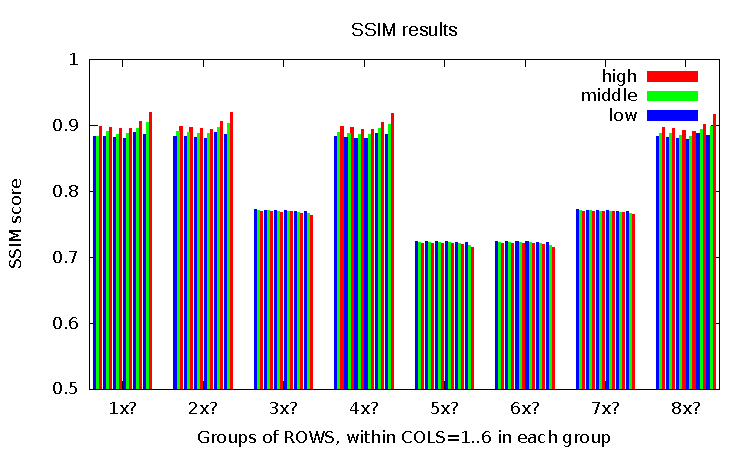
\includegraphics[width=.31\textwidth]{../figures/ssim.pdf}
		\label{fig:ssim}
	}	
	\caption{Evaluation results on a 30 second video with a resolution of $3840\times2048$ pixels. High and low bitrates are 1.6Mbps and 0.8Mbps, corresponding to 480p and 360p video, respectively.\protect\footnotemark}
	\label{fig:eval}
\end{figure*}
To evaluate RATS, we analyze its performance across multiple tile configurations. In particular, we consider the encoding speed, output file size, and the quality of the final image.
%
Examining Figs.~\ref{fig:time} and \ref{fig:size}, we see that the number of tile columns is the primary factor affecting encoder performance. Intuitively, this makes sense; the number of columns dictates the number of sub-images necessary, each of which requires two more NVENC encodes per frame, multiple stitching operations, and column stacking of the source image. In contrast, the hardware encoder supports tile rows using Slice mode. Slice mode incurs additional computation costs only when alignment rules force us to crop the source image.

Fig.~\ref{fig:time} confirms that RATS easily satisfies our real-time requirement, finishing the encode and stitch process in one-third of the total video time in the worst case tested.
The small jump from 1 to 2 columns is due to a required source image transformation, both before encoding and afterwards in stitching.
The larger jump from 4 to 5 columns happens when the stacked height reaches the hardware limit, and rearrangements are more severe because another hardware encoder instance is required.
The rapid increase thereafter happens within NVENC, obfuscating its origin.
It is likely a byproduct of the in-loop deblocking filter, which crosses tile boundaries but cannot do this efficiently in the increasingly tall and slim configurations. Configurations of 7 columns incur the worst case padding overhead, making it a particularly challenging case.

% The first notable point in the figure is the jump between 1 and 2 tile columns as the source image requires transformation and the stitcher begins to make more significant bitstream modifications. Another is the jump between 4 and 5 tile columns as sub-images are introduced.
% The gradual increase thenceforth occurs entirely within NVENC, unfortunately obfuscating its origin, but is likely a byproduct of the in-loop deblocking filter becoming less able to process tile boundaries in parallel as the image becomes taller and slimmer. The extra time at 7 columns similarly occurs within NVENC, and is likely due to the CTU width of the uncropped image not being divisible by 7, resulting in inferior alignment.

In Fig.~\ref{fig:size}, we see that the number of columns has a drastic effect on the output file size once sub-images are introduced. Decrease in coding efficiency is to be expected with smaller tiles due to intra-picture prediction and entropy encoding, but it is interesting that this only occurs with sub-images and is not affected by the number of tile rows.
This may also result from the in-loop deblocking filter.
As with Fig.~\ref{fig:time}, the spike at 7 columns is likely caused by inferior alignment.

In addition to having sufficient speed and coding efficiency, we must ensure that the video quality is good enough to achieve a high quality of experience for the end user.
In a tile-based ABR streaming scenario, this is especially true in high-quality tiles since these will likely be at the current position of the viewport.
Furthermore, NVENC is a new technology not yet capable of matching the output quality of software encoders, and we can expect quality to degrade with more tiles because intra-prediction and motion estimation cannot pass tile boundaries, so choosing an appropriate tile granularity is essential.
We use SSIM to express the deviation between the original and the tiled encoded frames, showing the results in Fig.~\ref{fig:ssim}.
Well-aligned tile configurations (1, 2, 4 and 8 rows, 1 through 6 colums) provide an intuitive quality degradation from high to low quality. Forced alignment of the tile height by cropping requires interpolation before SSIM, with the result that lower quality images with higher blur scores better in SSIM. Configurations with 7 and 8 columns require horizontal padding, resulting in very low SSIM scores.

\footnotetext{https://support.google.com/youtube/answer/2853702}



%\begin{figure}[t]
%	% \includegraphics[width=\columnwidth]{figures/hevc_eval_qual.png}
%	\caption{Encoding speed vs. tile quality for $4\times4$ tiles. All tiles on the left are of the high bitrate, while those on the right are of the low bitrate.}
%\end{figure}



%\begin{figure}[t]
%	\includegraphics[width=\columnwidth]{figures/times_v1.pdf}
	%\caption{Encoding time for a 30s video across tile configurations. The tile qualities alternate between high and low in a checkerboard pattern. For each configuration that has an odd number of tiles, we set the extra tile to be low quality.}
	%\label{fig:time}
%\end{figure}


%\begin{figure}[t]
%	\includegraphics[width=\columnwidth]{figures/sizes_v1.pdf}
%	\caption{Encoding output size in MB for a 30s video across tile configurations. The tile qualities alternate between high and low in a checkerboard pattern. }
%	\label{fig:size}
%\end{figure}

%\begin{figure}[t]
%	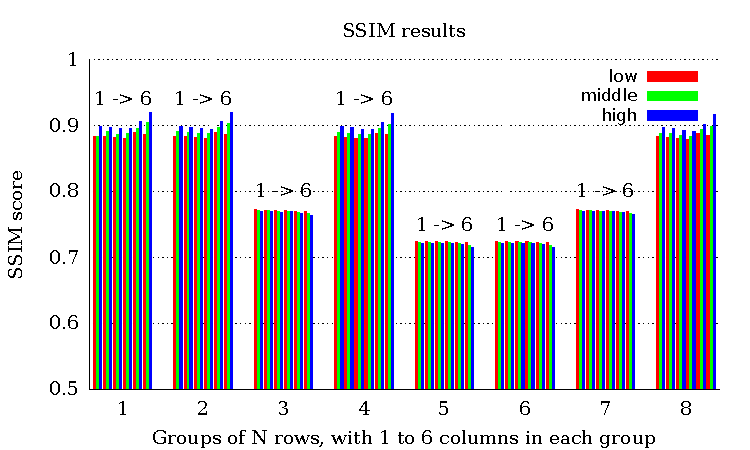
\includegraphics[width=\columnwidth]{figures/ssim.pdf}
%	\caption{Encoding output size in MB for a 30s video across tile configurations. The tile qualities alternate between high and low in a checkerboard pattern. }
%	\label{fig:ssim}
%\end{figure}

\section{Conclusion} \label{concl}

In this work, we demonstrated an adaptive live video platform capable of encoding tiled $360\,^{\circ}$ videos at multiple bitrates using an accessible consumer-grade GPU. By working closely with NVENCODE and the HEVC standard, we overcame limitations that had previously rendered hardware encoders useless in generating adaptive tile-based video. Furthermore, we have made our code open source and provided a demonstration of an HTTP video streaming service based on RATS.

%\begin{figure}[t]
%	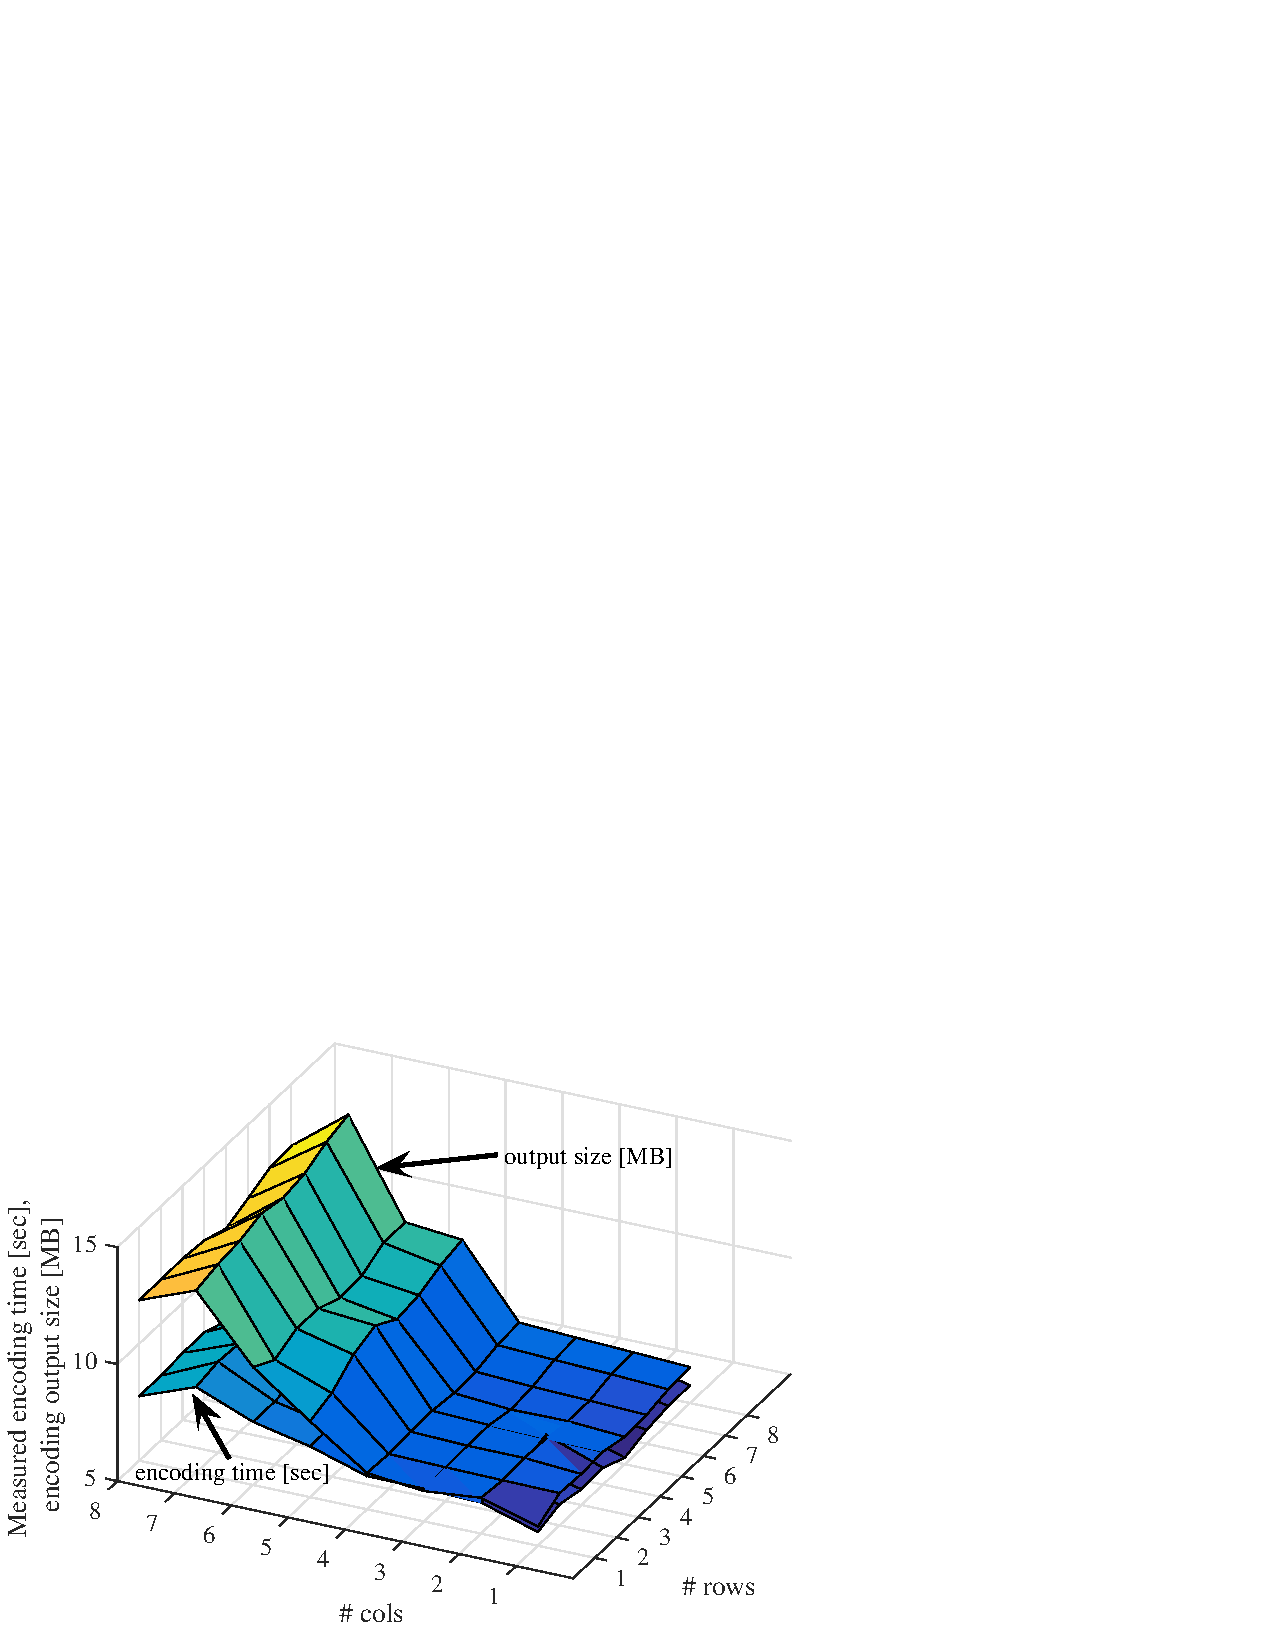
\includegraphics[width=\columnwidth]{figures/times_size_combined_v1.pdf}
%	\caption{JUST FOR US. A combined view of the encoding time and the resulting output size.}
%\end{figure}
